% Springer classic template (svjour3)
\documentclass{svjour3}

% Packages
\usepackage[utf8]{inputenc}
\usepackage[T1]{fontenc}
\usepackage{lmodern} % Latin Modern (T1) text fonts
\usepackage{fix-cm}  % allow arbitrary CM font sizes if CM is still used somewhere
\renewcommand{\rmdefault}{lmr}
\renewcommand{\sfdefault}{lmss}
\renewcommand{\ttdefault}{lmtt}
\usepackage{microtype}

% Quiet noisy but harmless log messages
\usepackage{silence}
\WarningFilter{latex}{Command \showhyphens has changed.}

% Math/theorems
\usepackage{amsmath,amssymb,mathtools}
% svjour3 provides its own theorem/proof support; keep AMS math only.

% Tables/figures
\usepackage{booktabs}
\usepackage{enumitem}
\usepackage{graphicx}
\usepackage{tikz}
\usetikzlibrary{arrows.meta,positioning}

% Citations (author--year)
\usepackage{natbib}
\setcitestyle{authoryear,round}
\usepackage{xurl}

% Links and cross-references
\usepackage[hidelinks]{hyperref}

% Author metadata
\usepackage{orcidlink}

% --- Springer svjour3 front matter ---
\title{Alluka Something Algorithmic Debt: A Formal View of Prompt Ambition, Verification Overhead, and Sequential Safety Cost}
\titlerunning{Algorithmic Debt in Prompted Inference}

\author{Aryan Singh Chandel\,\orcidlink{0009-0007-1774-2480}}
\authorrunning{A. S. Chandel}

\institute{Aryan Singh Chandel \at
  RJIT (Rustamji Institute of Technology), Gwalior, India \\
  \email{aryansingh19gh@gmail.com}
}

\journalname{Preprint}
\date{June 26, 2026}

% Theorems (svjour3) — only define if the class hasn't already
\makeatletter
\@ifundefined{definition}{\spnewtheorem{definition}{Definition}{\bfseries}{\rmfamily}}{}
\@ifundefined{assumption}{\spnewtheorem{assumption}{Assumption}{\bfseries}{\rmfamily}}{}
\@ifundefined{proposition}{\spnewtheorem{proposition}{Proposition}{\bfseries}{\itshape}}{}
\makeatother
\raggedbottom
\emergencystretch=3em

\begin{document}
\maketitle

\begin{abstract}
Token counts are an incomplete proxy for the operational cost of serving large language models. Prompts of comparable length can induce very different amounts of non-generation work, including retrieval, decomposition, verification, and safety filtering. We propose an explicit cost decomposition into generation, verification, and safety terms and define a normalized \emph{algorithmic debt} ratio that isolates overhead relative to base generation. We also introduce a length-controlled benchmarking protocol that stratifies prompts by annotated ambition---depth, breadth, and risk---and records stage-wise token, latency, and, when available, energy measurements. A small pilot study demonstrates the measurement workflow and motivates larger, pre-registered evaluations.
\keywords{Large language models \and Inference cost \and Verification \and Safety \and Benchmarking}
\end{abstract}

\section{Introduction}
Scaling-law studies connect model capability to training compute \cite{kaplan2020scaling,hoffmann2022chinchilla}. At deployment, however, the more immediate concern is end-to-end serving burden: how much work a system performs at inference time, how that work is staged, and which parts of it are triggered by the prompt itself \cite{wu2024inferencescaling,tokenbudget2024}. In long-context settings, more input can even degrade performance by introducing retrieval and positional failure modes rather than monotone gains \cite{liu2023lost}. These observations motivate separating raw input length from prompt-induced operational overhead.

In practice, prompts with similar token length can require very different serving pipelines: repeated attempts, auxiliary verification stages, external tool calls, or safety-motivated rewrites. Token accounting alone therefore conflates base generation with downstream orchestration. We formalize that excess burden as \emph{algorithmic debt} and propose a measurement framework intended to be comparable across models and serving stacks.

\paragraph{Contributions.} This paper:
\begin{enumerate}[leftmargin=*]
\item introduces an operational cost decomposition $C_{\text{total}}=C_{\text{gen}}+C_{\text{ver}}+C_{\text{safe}}$ and a normalized algorithmic-debt ratio;
\item defines ambition annotations (depth, breadth, and risk) and a length-controlled stratification scheme to separate verbosity from complexity;
\item specifies a logging protocol and estimands for evaluating how ambition predicts non-generation overhead; and
\item reports a small pilot measurement to demonstrate the end-to-end workflow.
\end{enumerate}

\section{Model and estimands}
\subsection{Cost decomposition}
Let $x$ denote a prompt instance under a fixed serving configuration (model, decoding parameters, stage policy, and hardware/runtime). We decompose the total serving burden into
\[
C_{\text{total}}(x)=C_{\text{gen}}(x)+C_{\text{ver}}(x)+C_{\text{safe}}(x),
\]
where $C_{\text{gen}}$ is the base generation burden and $C_{\text{ver}}$ and $C_{\text{safe}}$ capture non-generation overhead from verification and safety processes. Each component may be measured in tokens, latency, or energy; throughout, the unit must be reported together with the serving configuration.

\begin{table}[t]
\caption{Core notation used throughout the paper.}
\label{tab:notation}
\centering
\begin{tabular}{ll}
\toprule
Symbol & Meaning \\
\midrule
$x$ & prompt instance \\
$C_{\text{gen}}(x)$ & base generation burden \\
$C_{\text{ver}}(x)$ & verification/checking overhead \\
$C_{\text{safe}}(x)$ & safety/alignment overhead \\
$W(x)$ & ambition score (definition below) \\
$AD(x)$ & algorithmic debt ratio \\
$SR(x)$ & sequential request burden \\
$m(x)$ & number of auxiliary stages \\
\bottomrule
\end{tabular}
\end{table}

\subsection{Ambition and algorithmic debt}
\begin{definition}[Wish complexity]
The ambition (wish complexity) of prompt $x$ is
\[
W(x)=\alpha L(x)+\beta D(x)+\gamma B(x)+\delta R(x),
\]
where $L$ is normalized input length, $D$ is reasoning depth, $B$ is conceptual breadth, and $R$ is safety sensitivity.
\end{definition}

\begin{definition}[Algorithmic debt]
Define the algorithmic debt ratio as
\[
AD(x)=\frac{C_{\text{ver}}(x)+C_{\text{safe}}(x)}{C_{\text{gen}}(x)+\varepsilon},
\]
for a small $\varepsilon>0$.
\end{definition}

\begin{definition}[Sequential request burden]
Let $m(x)$ be the number of auxiliary checks, clarification rounds, or guardrail stages required before a response is accepted. The sequential request burden is
\[
SR(x)=\sum_{s=1}^{m(x)} c_s(x),
\]
where $c_s(x)$ is the measured cost of stage $s$ in the chosen unit.
\end{definition}

\begin{definition}[Marginal debt elasticity]
Within a fixed serving configuration, define the marginal debt elasticity of ambition as
\[
\mathcal{E}_{AD,W}(x)=\frac{\partial \log(AD(x)+1)}{\partial \log(W(x)+1)}.
\]
This quantity distinguishes systems in which additional ambition produces roughly proportional overhead from systems in which overhead accelerates sharply.
\end{definition}

\subsection{Assumptions (measurement)}
Our goal is not to assert a mechanistic model of serving stacks, but to define estimands that can be measured under a declared protocol. We assume:
\begin{enumerate}[leftmargin=*]
\item \textbf{Cost separability:} $C_{\text{gen}}$, $C_{\text{ver}}$, and $C_{\text{safe}}$ can be estimated from logs with acceptable measurement error.
\item \textbf{Ambition heterogeneity:} prompts of comparable length can vary materially in $D(x)$, $B(x)$, and $R(x)$.
\item \textbf{Operational relevance:} non-generation overhead is reflected in observable cost units (latency, energy, or auxiliary-token additions) rather than only in internal bookkeeping.
\end{enumerate}

\subsection{Primary estimand and hypothesis}
The primary estimand is the association between ambition and debt under length control. Concretely, within narrow length strata (or with an explicit length covariate), we estimate the slope
\[
T_A = \hat{\beta}_{W\rightarrow AD}.
\]
The null hypothesis is $T_A\le 0$, i.e., after controlling for length, ambition does not predict additional non-generation overhead.

An operational regression form is
\[
AD(x)=\beta_0+\beta_1W(x)+\beta_2L(x)+\beta_3Z(x)+\varepsilon_x,
\]
where $Z(x)$ collects declared confounds such as domain, retrieval dependence, or policy mode. The core empirical question is whether $\beta_1$ remains positive after these adjustments.

\subsection{Secondary estimands}
Two secondary quantities matter for interpretation. First, we estimate stage-share ratios
\[
\rho_{\mathrm{ver}}(x)=\frac{C_{\mathrm{ver}}(x)}{C_{\mathrm{total}}(x)},
\qquad
\rho_{\mathrm{safe}}(x)=\frac{C_{\mathrm{safe}}(x)}{C_{\mathrm{total}}(x)},
\]
which localize where the debt originates. Second, we estimate the within-bin rank correlation between $W(x)$ and $AD(x)$ to test whether the theory survives without assuming linearity.

\subsection{Stratified estimation}
Let $\mathcal{B}$ denote length bins. A length-controlled aggregate slope may be estimated by
\[
\widehat{\beta}_{\mathrm{strat}}=
\sum_{b\in\mathcal{B}}\omega_b\,\widehat{\beta}_b,
\qquad
\omega_b=\frac{n_b}{\sum_{b'}n_{b'}},
\]
where $\widehat{\beta}_b$ is the within-bin slope of $AD$ on $W$. This avoids treating length control as purely parametric when prompt distributions are irregular.

\subsection{Monotonicity test statistic}
If the theory is interpreted as an ordered-overhead claim, a simple nonparametric statistic is
\[
T_{\uparrow}=
\frac{1}{|\mathcal{P}|}
\sum_{(x_i,x_j)\in\mathcal{P}}
\mathbf{1}\{W(x_i)>W(x_j),\ AD(x_i)>AD(x_j)\},
\]
where $\mathcal{P}$ is the set of length-matched prompt pairs. Values near $1/2$ indicate no systematic ordering beyond chance, whereas large values support monotone debt growth with ambition.

\subsection{Inference and calibration}
Uncertainty should be reported through prompt-family bootstrap resampling or by clustered standard errors when repeated prompts share templates or annotation pipelines. In addition, the ambition summary variable should be calibrated against its components by checking whether
\[
\operatorname{Var}\!\bigl(AD(x)\mid W(x)\bigr)
\]
is materially larger than
\[
\operatorname{Var}\!\bigl(AD(x)\mid L(x),D(x),B(x),R(x)\bigr).
\]
If the latter variance drops sharply, the scalar summary is too compressive and should not dominate interpretation.

\subsection{Benchmark design (summary)}
To avoid conflating verbosity with ambition, prompt families are constructed to be approximately length-matched while varying annotated depth $D(x)$, breadth $B(x)$, and risk $R(x)$. The benchmark records stage-wise costs (tokens, latency, and optionally energy) and stage outcomes (accepted, revised, blocked).

The detailed annotation rubric, endpoint definitions, reproducibility checklist, stage taxonomy, and confound checklist are provided in Appendix~A.

\subsection{Threats to validity (summary)}
A central threat is misattribution: retrieval failures, context-window pathologies, or infrastructure latency may be incorrectly counted as verification overhead. Our protocol therefore requires explicit logging of stage triggers and, where applicable, retrieval events, together with sensitivity analyses that exclude dominated failure modes. Since the framework is empirical, evidence must be based on replicated measurements under declared configurations rather than on first-principles arguments about any particular serving system.

Another threat is construct compression. If $W(x)$ is too coarse, then depth, breadth, and risk can trade off against one another in ways that flatten the observed signal. For that reason, the paper treats $W(x)$ as a benchmarked summary variable rather than an untouchable primitive; a serious evaluation should also report its components separately.

A further methodological risk is post hoc stage definition. If verification and safety stages are defined after seeing the logs, debt estimates become researcher degrees of freedom. The stage taxonomy should therefore be frozen before benchmark execution.

\begin{figure}[t]
\centering
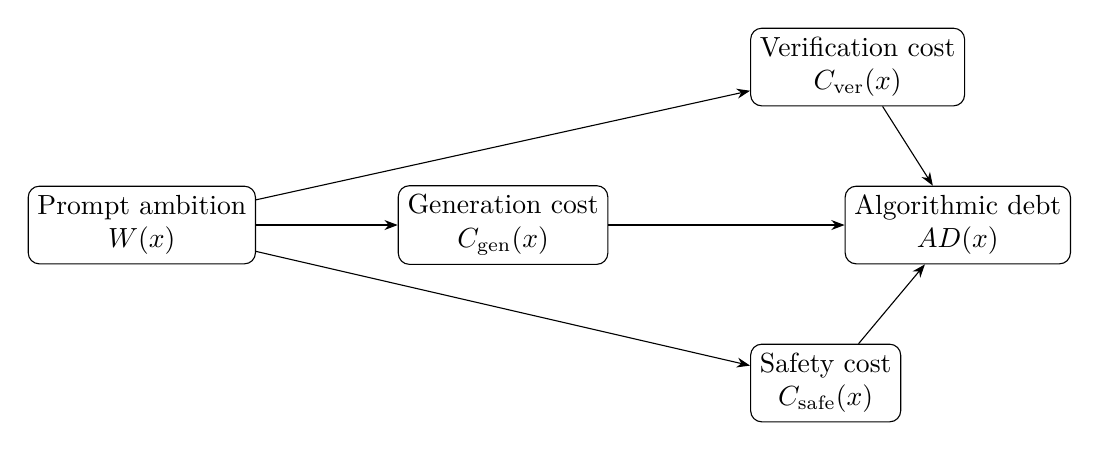
\begin{tikzpicture}[node distance=1.8cm,>=Stealth]
\node[draw,rounded corners,align=center] (w) {Prompt ambition\\$W(x)$};
\node[draw,rounded corners,right=of w,align=center] (g) {Generation cost\\$C_{\text{gen}}(x)$};
\node[draw,rounded corners,above right=1.0cm and 1.8cm of g,align=center] (v) {Verification cost\\$C_{\text{ver}}(x)$};
\node[draw,rounded corners,below right=1.0cm and 1.8cm of g,align=center] (s) {Safety cost\\$C_{\text{safe}}(x)$};
\node[draw,rounded corners,right=3.0cm of g,align=center] (a) {Algorithmic debt\\$AD(x)$};
\draw[->] (w) -- (g);
\draw[->] (w) -- (v);
\draw[->] (w) -- (s);
\draw[->] (g) -- (a);
\draw[->] (v) -- (a);
\draw[->] (s) -- (a);
\end{tikzpicture}
\caption{Cost-decomposition view of algorithmic debt. The central claim is that prompt ambition can increase verification and safety overhead even when base generation remains modest.}
\label{fig:alluka-decomposition}
\end{figure}

\section{Related Work}
Training-time scaling laws motivate the broader question of regularities between compute and capability \cite{kaplan2020scaling,hoffmann2022chinchilla}. Inference-side studies show that additional test-time computation can change the quality--cost frontier \cite{wu2024inferencescaling,tokenbudget2024}. Long-context evaluations warn that larger context windows introduce failure modes that can reduce utility \cite{liu2023lost}. Energy and latency profiling further connect workload characteristics to measurable serving cost \cite{husom2024price}. Our contribution differs in focusing on a prompt-induced overhead decomposition intended to be measured under length control.

\begin{figure}[t]
\centering
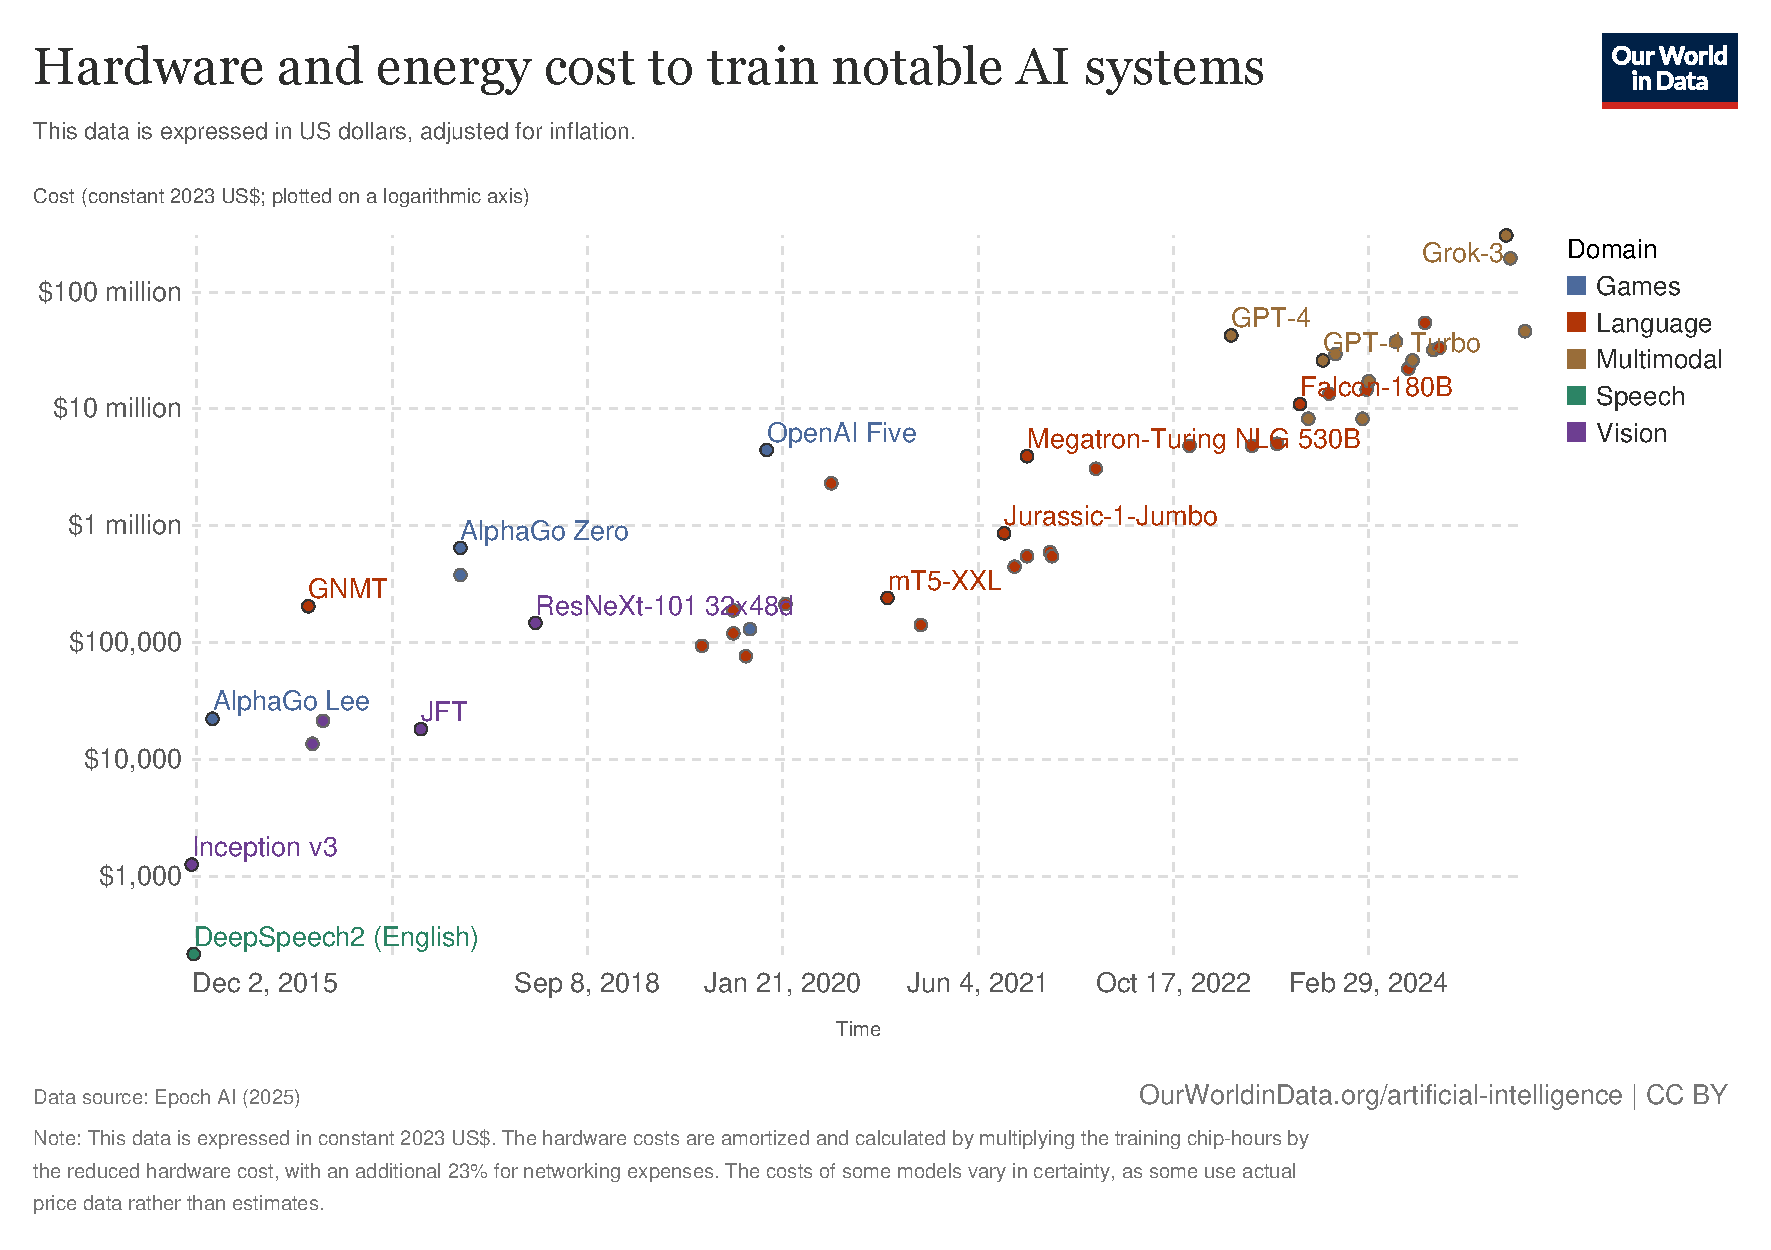
\includegraphics[width=\linewidth]{figures/owid_hardware_energy_costs.pdf}
\caption{Broader AI cost growth context from Our World in Data, adapted from Epoch AI and released under CC BY \citep{owid_hardware_energy_costs}. This figure does not measure our proposed debt ratio directly, but it motivates why operational cost accounting matters.}
\label{fig:alluka-owid}
\end{figure}

\section{Pilot study (seed measurement)}
\subsection{Setup}
We conducted a pilot measurement to validate that the proposed logging and decomposition can be executed end-to-end. The pilot used nine public prompts spanning factual extraction, arithmetic reasoning, and medical multiple-choice questions. All runs used \texttt{google/flan-t5-small} under a fixed decoding and runtime configuration.

\subsection{Measurement unit}
In the pilot, cost components were operationalized as stage-wise token counts. Verification and safety stages were invoked only when required by the benchmark metadata (i.e., the stage policy was externally specified rather than adaptively learned).

\subsection{Aggregate result}
Table~\ref{tab:alluka-seed} reports the pilot aggregate for a single prompt family.
\begin{table}[t]
\centering
\begin{tabular}{lccccc}
\toprule
Family & Mean $W$ & Mean $C_{\text{gen}}$ & Mean $C_{\text{ver}}$ & Mean $C_{\text{safe}}$ & Mean $AD$ \\
\midrule
\texttt{alluka\_public\_seed} & 0.5133 & 106.7778 & 59.0000 & 26.3333 & 1.5637 \\
\bottomrule
\end{tabular}
\caption{Pilot (seed) cost decomposition measured on public benchmark prompts using stage-wise token counts.}
\label{tab:alluka-seed}
\end{table}



\begin{table}[t]
\centering
\caption{Seed-scale mean cost decomposition by prompt group.}
\label{tab:alluka-groups}
\begin{tabular}{lcccc}
\toprule
Group & Mean $C_{\text{gen}}$ & Mean $C_{\text{ver}}$ & Mean $C_{\text{safe}}$ & Mean $AD$ \\
\midrule
SQuAD & 204.0 & 0.0 & 0.0 & 0.0000 \\
GSM8K & 66.3 & 102.0 & 0.0 & 1.5404 \\
MedMCQA & 50.0 & 75.0 & 79.0 & 3.1508 \\
\bottomrule
\end{tabular}
\end{table}

\begin{figure}[t]
\centering
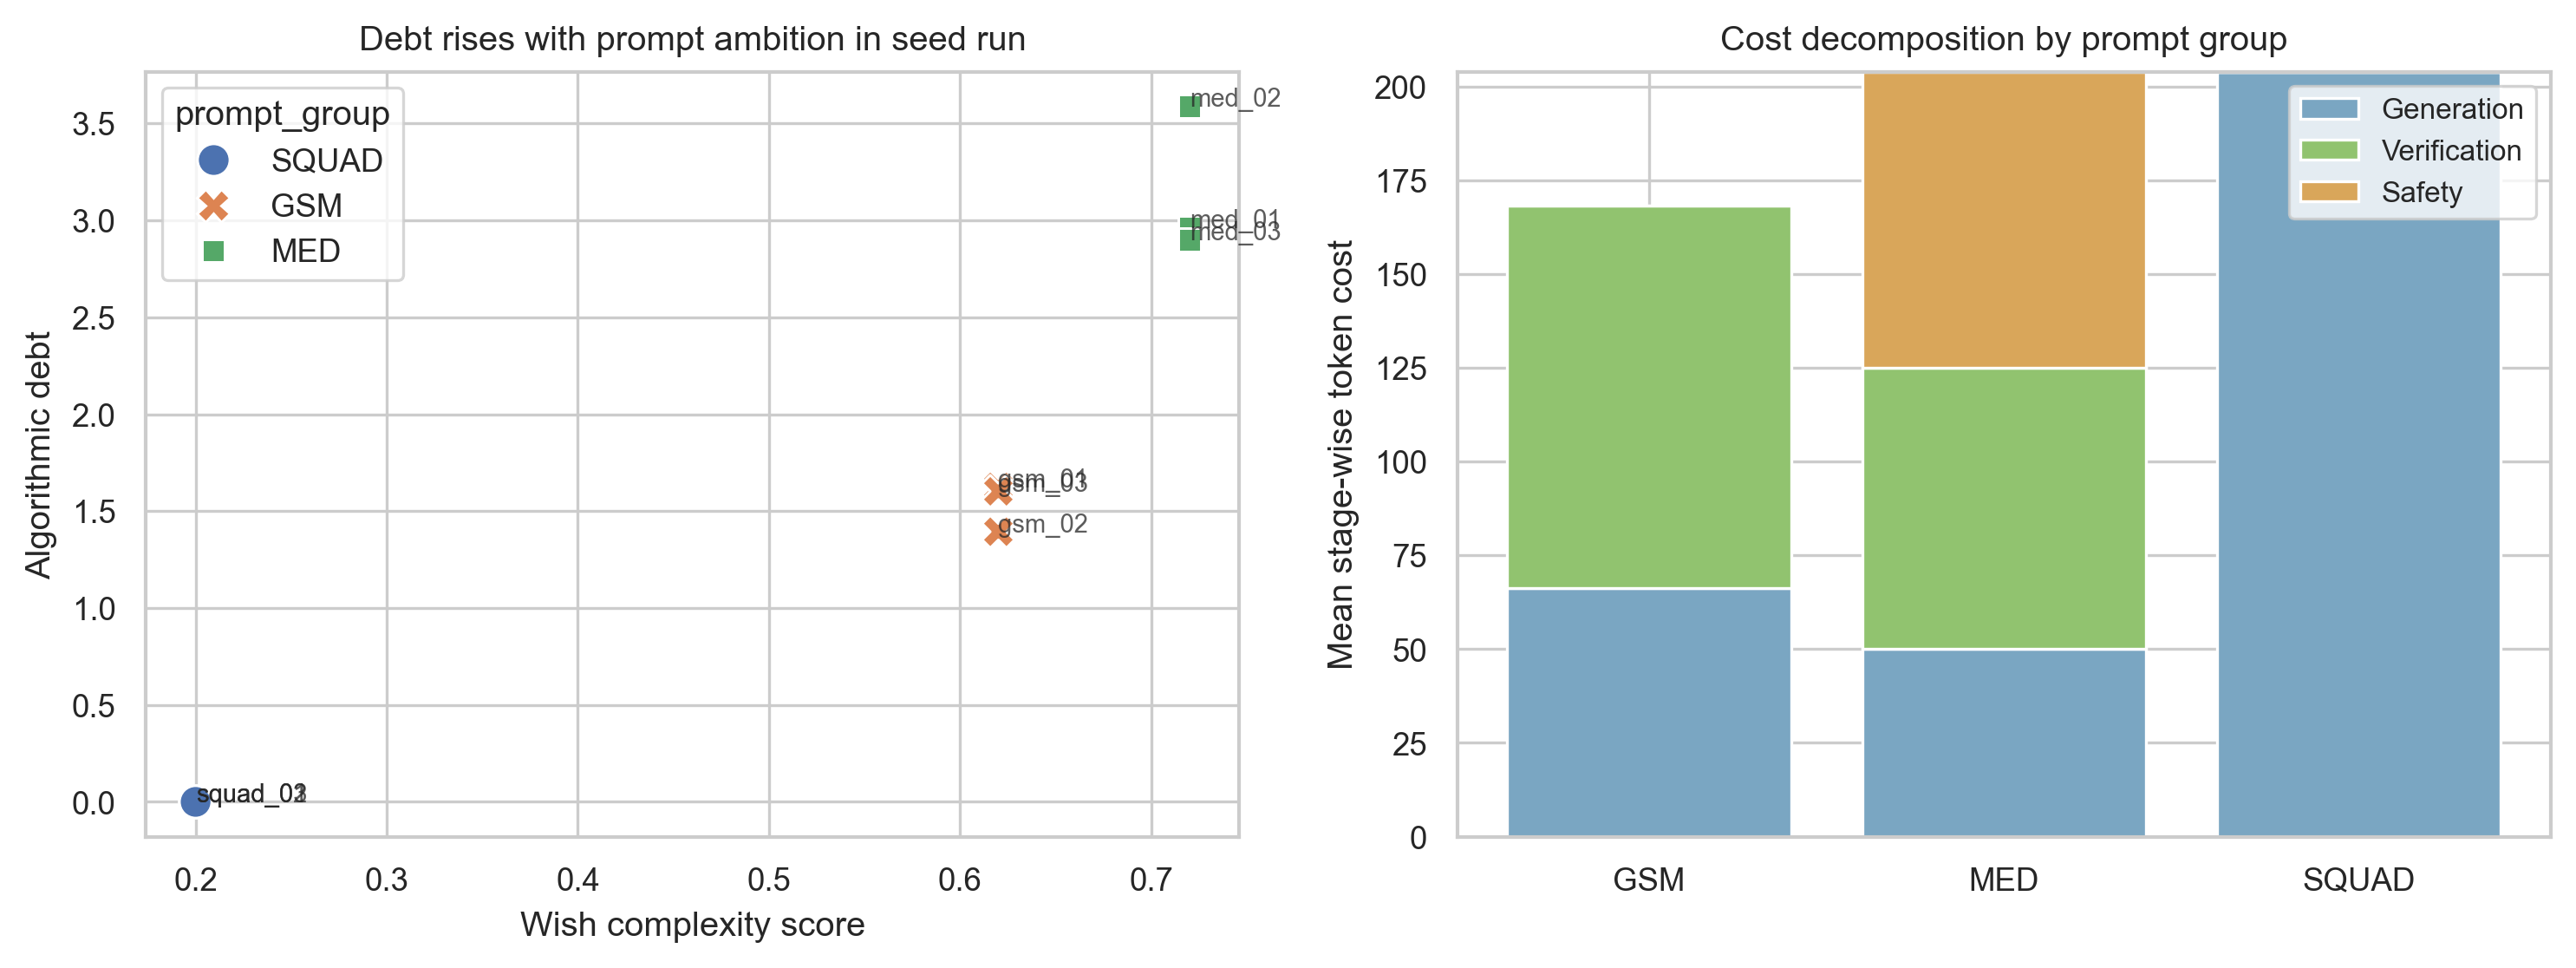
\includegraphics[width=\linewidth]{figures/alluka_seed_results.png}
\caption{Measured seed-scale behavior. Left: algorithmic debt against annotated wish complexity. Right: mean stage-wise token cost by prompt group.}
\label{fig:alluka-seed}
\end{figure}

\subsection{What is learned}
The pilot indicates that, even for a small set of prompts, non-generation stages can contribute materially to total serving burden and can exceed base generation in the chosen unit. This supports the methodological claim that separating $C_{\text{gen}}$, $C_{\text{ver}}$, and $C_{\text{safe}}$ is practically relevant and measurable.

The group-level pattern is also directionally informative. In the current pilot, the progression from SQuAD to GSM8K to MedMCQA is not merely a change in prompt length; it is a change in the amount of verification and safety machinery recruited around the base generator. That is exactly the distinction the debt framework is designed to expose.

\subsection{What is not claimed}
The pilot is not a scaling result and does not establish a universal relationship between $W(x)$ and $AD(x)$. The sample size is too small for stable inference, and token accounting alone does not capture hardware- and system-dependent costs such as latency or energy. The pilot therefore serves only as a feasibility check for instrumentation and reporting; substantive conclusions require larger, pre-registered prompt families and replication across models and serving stacks.

In particular, the pilot does not identify a universal elasticity parameter. Any claim about superlinear debt growth would require repeated measurements across ambition strata, explicit confidence intervals for $\mathcal{E}_{AD,W}$, and replication across serving policies.

\section{Discussion}
The main contribution of the paper is not a fitted law but a cleaner accounting language. Once generation, verification, and safety are reported separately, it becomes possible to ask more precise questions about where operational burden originates and which prompt properties actually induce it. That shift matters because many discussions of inference cost still treat token length as the dominant explanatory variable even when deployment stacks impose additional stages that are only loosely correlated with length.

The pilot also suggests a useful interpretive distinction. Some prompts are expensive because they are long; others are expensive because they recruit machinery around the model. The latter class is the one the algorithmic-debt framing is designed to expose. Whether the proposed ambition score is the best predictor remains open, but the decomposition itself already makes evaluation more informative.

That distinction also has reporting consequences. If inference studies publish only input length and final latency, then verification-heavy and safety-heavy workloads can look deceptively similar to straightforward generation. A stage-aware accounting scheme makes it easier to compare systems that solve the same surface task with very different internal burdens.

The more ambitious version of the theory is therefore not ``big prompts cost more.'' That statement is too weak to be interesting. The sharper claim is that, after length is controlled, prompts differing in inferential depth, breadth, and policy sensitivity can induce systematically different non-generation burdens, and that these burdens can be decomposed in a reproducible way. The present pilot does not prove that claim, but it does make the claim empirically legible.

\section{Limitations and Future Work}
This manuscript reports only a small seed study and proposes a measurement framework rather than a validated scaling law. Four limitations matter most. First, the current sample is too small for stable effect estimation. Second, the pilot uses one serving configuration and therefore cannot separate model-specific behavior from broader regularities. Third, token counts are only one cost unit; latency and energy must be incorporated before strong operational claims can be made. Fourth, the ambition annotations themselves remain partly judgment-based and will require stronger inter-annotator or rubric-based validation.

Immediate next steps are straightforward: expand the prompt families, pre-register the strata, replicate across open- and closed-weight systems, and report tokens, latency, and energy jointly wherever feasible. A stronger version of the paper would also test whether ambition predicts debt after explicitly controlling for domain, retrieval dependence, and safety policy mode.

\section{Conclusion}
If algorithmic debt is real, prompt design should be evaluated the way systems engineers evaluate hidden coupling: not by how dramatic the request sounds, but by how much extra machinery it quietly forces into the loop.

\appendix
\section{Supplementary benchmark specification}
This appendix collects protocol details that are referenced in the main text.

\subsection{Annotated variables and endpoints}
\begin{table}[t]
\centering
\caption{Annotated benchmark variables used to score prompt ambition and to stratify prompt families.}
\label{tab:bench-variables}
\small
\begin{tabular}{@{}p{0.22\linewidth}p{0.15\linewidth}p{0.55\linewidth}@{}}
\toprule
Variable & Symbol & Interpretation \\
\midrule
Prompt length & $L(x)$ & Tokenized input size after normalization \\
Reasoning depth & $D(x)$ & Number of dependent inferential steps required \\
Conceptual breadth & $B(x)$ & Number of distinct domains or constraints involved \\
Safety sensitivity & $R(x)$ & Degree of policy, risk, or verification pressure \\
Debt ratio & $AD(x)$ & Non-generation overhead relative to base generation \\
\bottomrule
\end{tabular}
\end{table}

\begin{table}[t]
\centering
\caption{Primary measured endpoints and their role in the decision rule.}
\label{tab:bench-endpoints}
\small
\begin{tabular}{@{}p{0.24\linewidth}p{0.18\linewidth}p{0.50\linewidth}@{}}
\toprule
Endpoint & Symbol & Decision role \\
\midrule
Generation cost & $C_{\text{gen}}$ & Baseline denominator \\
Verification cost & $C_{\text{ver}}$ & Captures checking overhead \\
Safety cost & $C_{\text{safe}}$ & Captures alignment overhead \\
Debt ratio & $AD(x)$ & Primary normalized endpoint \\
Sequential burden & $SR(x)$ & Captures multi-stage orchestration load \\
\bottomrule
\end{tabular}
\end{table}

\subsection{Reproducibility checklist}
\begin{table}[t]
\centering
\caption{Reproducibility checklist for an algorithmic-debt measurement run (implementation-agnostic).}
\label{tab:repro-checklist}
\small
\begin{tabular}{@{}p{0.24\linewidth}p{0.68\linewidth}@{}}
\toprule
Category & Minimum information to report \\
\midrule
Model identity & Model name, revision/hash (if available), context length, tokenizer version \\
Decoding & Temperature, top-$p$, max output tokens, stop conditions, any constraints \\
Stage policy & Stage types enabled, triggers, max stages $m(x)$, accept/reject criteria \\
Cost units & Tokens (in/out per stage), latency (per stage + end-to-end), optional energy \\
Hardware/runtime & Device type, precision, batch size, framework + version \\
Randomness & Seeds (where applicable), number of repeated runs per prompt \\
Logging & Timestamps, per-stage metadata, tool-call flags, caching on/off \\
Prompt release & Prompt families + annotations, or a clear access/availability statement \\
\bottomrule
\end{tabular}
\end{table}

\subsection{Stage taxonomy}
\begin{table}[t]
\centering
\caption{Stage taxonomy for logging and for separating generation from non-generation overhead.}
\label{tab:stage-taxonomy}
\small
\begin{tabular}{@{}p{0.16\linewidth}p{0.30\linewidth}p{0.46\linewidth}@{}}
\toprule
Stage type & Typical trigger (observable) & What to log (minimum) \\
\midrule
Generation & Response requested; decoding begins & Input/output tokens, latency, decoding parameters, cache hits \\
Verification & Factuality/consistency required; check invoked & Check method (tool/self-check), number of checks, added tokens, latency \\
Safety & Policy risk elevated; filter/classifier invoked; refusal/rewrites possible & Policy mode, classifier decision, block/allow, rewrites, added tokens/latency \\
\bottomrule
\end{tabular}
\end{table}

\subsection{Common confounds}
\begin{table}[t]
\centering
\caption{Common confounds and mitigations when estimating algorithmic debt under length control.}
\label{tab:confounds}
\small
\begin{tabular}{@{}p{0.28\linewidth}p{0.28\linewidth}p{0.36\linewidth}@{}}
\toprule
Confound & Symptom in logs & Mitigation (protocol-level) \\
\midrule
Long prompt, trivial reasoning & High tokens, low stage count; low variance across runs & Add independent $D(x)$ annotation; include easy baselines within each length bin \\
Short prompt, hidden expertise & Low tokens but high $C_{\text{ver}}$ from repeated checks & Annotate domain difficulty; stratify by topic; report per-family debt \\
Infra latency (non-model) & Spikes in wall-clock without token increases & Separate token and latency metrics; record system load; repeat runs \\
Retrieval/pathology misattributed to verification & Verification stages triggered by missing/contradictory context & Log retrieval events separately; exclude known context-window failures in sensitivity analysis \\
\bottomrule
\end{tabular}
\end{table}

\section{Prompt Family Template (Reporting Checklist)}
\begin{table}[t]
\centering
\begin{tabular}{p{0.22\linewidth}p{0.70\linewidth}}
\toprule
Item & What to report for each prompt family \\
\midrule
Family ID & Stable identifier and a one-line description \\
Length control & Input token bin or matching rule \\
Depth $D(x)$ & Annotation rubric + example prompt(s) \\
Breadth $B(x)$ & Domains/constraints counted and rubric \\
Risk $R(x)$ & Safety/verification triggers and rubric \\
Stages & Allowed stage types and max stages $m(x)$ \\
Metrics & Tokens, latency, optional energy; how aggregated \\
Release & Whether prompts/logs are shared (and where) \\
\bottomrule
\end{tabular}
\caption{Minimum reporting checklist to make debt measurements comparable across systems.}
\label{tab:checklist}
\end{table}

\begin{figure}[t]
\centering
\resizebox{\linewidth}{!}{%
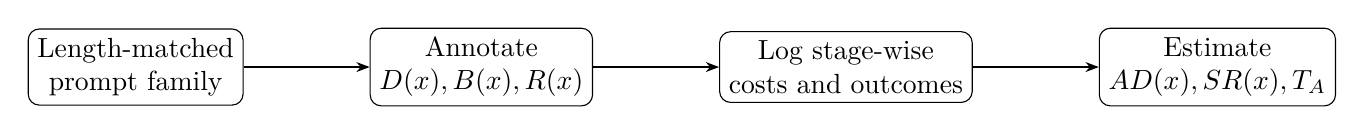
\begin{tikzpicture}[node distance=1.6cm,>=Stealth]
\node[draw,rounded corners,align=center] (p) {Length-matched\\prompt family};
\node[draw,rounded corners,right=of p,align=center] (a) {Annotate\\$D(x),B(x),R(x)$};
\node[draw,rounded corners,right=of a,align=center] (l) {Log stage-wise\\costs and outcomes};
\node[draw,rounded corners,right=of l,align=center] (r) {Estimate\\$AD(x),SR(x),T_A$};
\draw[->] (p) -- (a);
\draw[->] (a) -- (l);
\draw[->] (l) -- (r);
\end{tikzpicture}
}
\caption{Reporting workflow for a debt-measurement study. The emphasis is on separating ambition annotation from downstream operational logging.}
\label{fig:alluka-workflow}
\end{figure}

% --- Declarations / end-matter (journal-dependent; keep concise) ---
% (No acknowledgements.)

\section*{Declarations}
\paragraph{Funding} No external funding was received for this work.
\paragraph{Competing interests} The author declares no competing interests.
\paragraph{Data and materials availability} The data supporting the findings of this study are available from the corresponding author upon reasonable request.
\paragraph{Code availability} The code used for measurement is available from the corresponding author upon reasonable request.
\paragraph{Author contributions} Aryan Singh Chandel: conceptualization, methodology, writing---original draft, writing---review and editing.

\bibliographystyle{spbasic}
\bibliography{references}
\end{document}
